\section{Bedienungsanleitung}
Neben den in der Aufgabenstellung geforderten Funktionen der Anwendung wurden
einige vorgeschlagene Zusatzfunktionen implementiert:
\begin{itemize}
  \item Erkennung von Unbeschränktheit beim Aufbau des pEG
  \item Multiple Document Interface
  \item Übersichtliche Darstellung des pEG
\end{itemize}
Diese und darüber hinausgehende Funktionen der Anwendung werden in den folgenden
Unterabschnitten beschrieben.

\subsection{Tab Interface}
Die Untersuchung und Bearbeitung von mehreren Petri-Netzen gleichzeitig ist mit
Petri-Check durch ein Tab Interface ermöglicht. Jedes Petri-Netz wird dabei in
einem eigenen Tab, wie in modernen Web-Browsern, angezeigt.

Nach dem Start von PetriCheck wird dem Anwendy die in \cref{img:default_window}
gezeigte Bedienoberfläche präsentiert.

\begin{figure}[ht]
  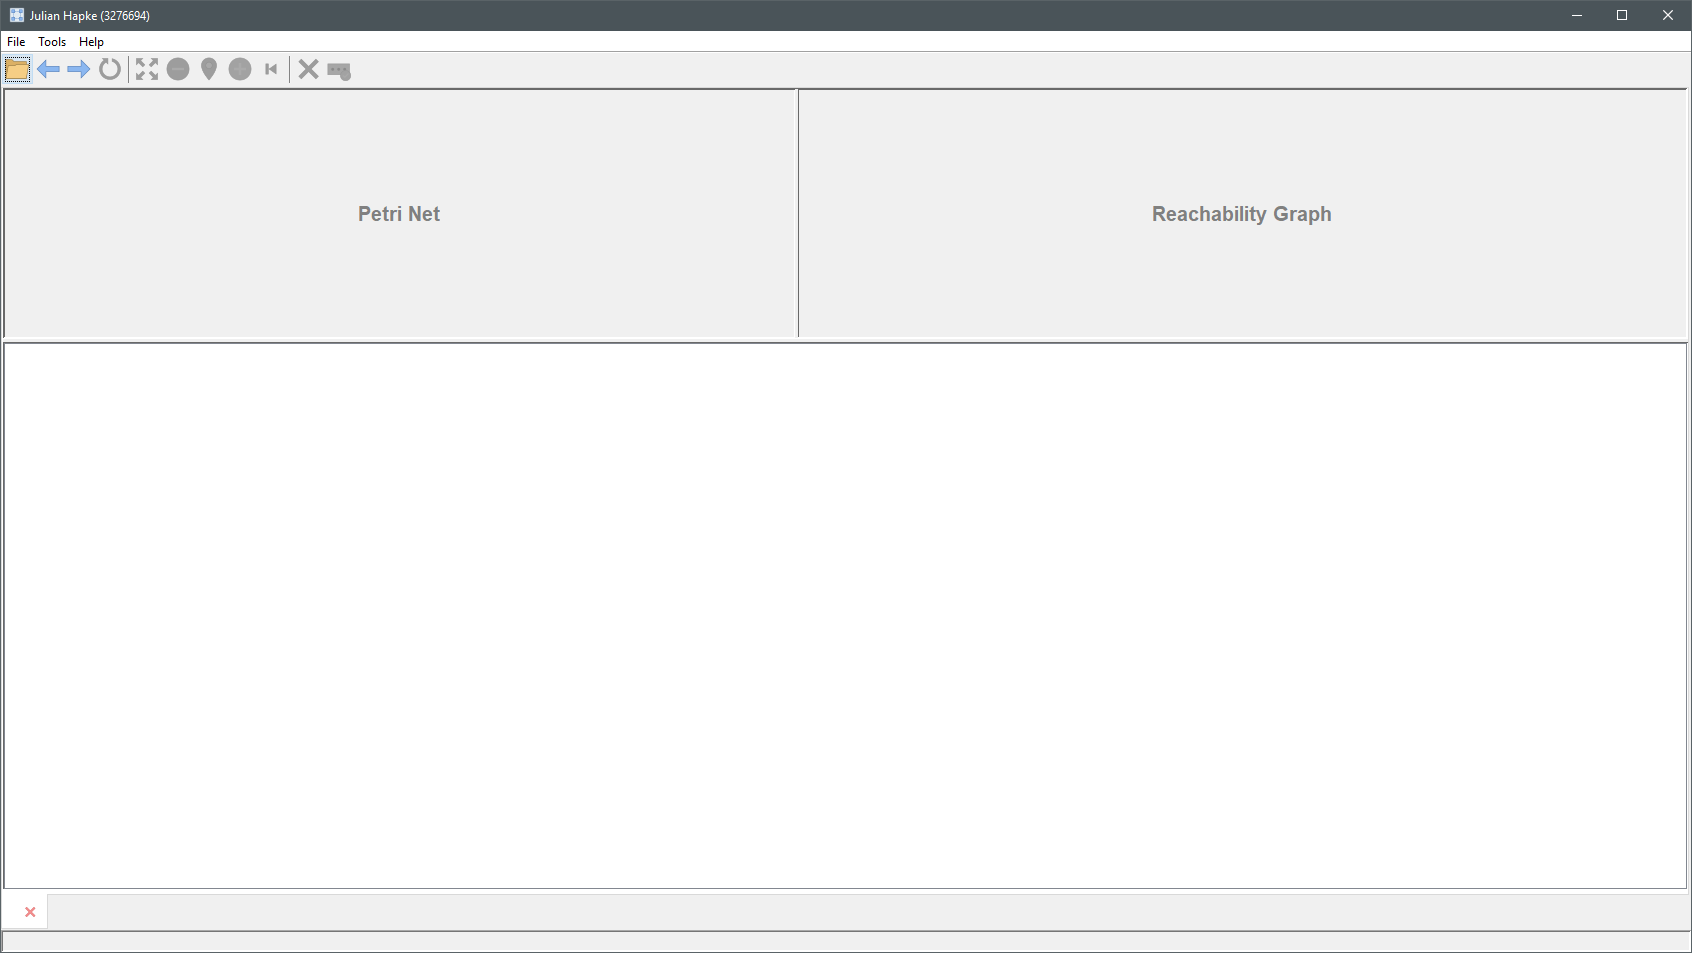
\includegraphics[width=\textwidth]{../img/default_window.png}
  \caption{Programmfenster nach dem Start}
  \label{img:default_window}
\end{figure}

Es ist kein Petri-Netz geöffnet, es wird aber ein Default-Tab angeboten, der
über einen vergrößerten Textausgabebereich verfügt. Dieser Bereich ist für die
Ausgabe der Ergebnisse einer Beschränktheitsanalyse mehrerer Dateien vorgesehen,
die auch ausgeführt werden kann, wenn kein Petri-Netz geöffnet ist.

Wird über die Standardfunktionen nun ein Petri-Netz geöffnet, so wird der
Default-Tab ersetzt, sofern in ihm keine Informationen im Textausgabebereich
vorhanden sind. Andersfalls wird ein zusätzlicher Tab erstellt.

Wegen der Möglichkeit mehrere Dateien gleichzeitig zu öffnen, ist in jedem
Dateiauswahldialog eine Mehrfachauswahl von PNML-Dateien möglich. Jede Datei
wird dann in einem eigenen Tab geöffnet. Ist eine ausgewählte Datei bereits
geöffnet, wird sie nicht erneut geöffnet, sondern der mit dieser Datei
assoziierte Tab aktiviert.

Um einen Tab und das darin enthaltene Petri-Netz zu schließen, existiert
einerseits der Menüpunkt \emph{Datei $\rightarrow$ Schließen}. Andererseits
verfügt jeder Tab am unteren Rand rechts neben seinem Titel über einen kleinen
\raisebox{-2pt}{
\includegraphics{../../src/main/resources/icons/icons8-delete-12.png}}
Button. Ein Klick auf diesen Button verursacht ebenfalls das Schließen des
entsprechenden Tabs. Wird jedoch der letzte Tab geschlossen, wird standardmäßig
ein leerer Default-Tab, wie in \cref{img:default_window} dargestellt, erzeugt,
um eine Ausgabemöglichkeit für die Stapelverarbeitung mehrerer Dateien zu haben.

\subsection{Mehrsprachigkeit}
Die Sprache der Bedienoberfläche kann verändert werden (siehe
\cref{sec:settings}). Beim ersten Start der Anwendung, wenn noch keine
Einstellung vorhanden ist, wird versucht die Sprache des Betriebssystems
einzustellen. Sind für diese Sprache keine Übersetzungsdateien vorhanden, wird
eine Oberfläche mit englischen Texten erstellt.

\subsection{Look and Feel}
Um eine im Vergleich zum Betriebssystem einheitliche Optik zu erreichen,
versucht PetriCheck das Look-and-Feel des Swing Frameworks an das des
Betriebssystems anzupassen. Nur wenn diese Anpassung scheitert, weil Swing z.B.
das aktuelle Betriebssystem nicht unterstützt, dient die etwas historisch
anmutende Standardoptik von Swing als Rückfallebene.

\subsection{Kontinuierliche Beschränktheitsanalyse}
Ein Anwendy kann während des interaktiven Schaltens über die Unbeschränktheit
des aktuellen Petri-Netzes informiert werden. Um diese Warnung nicht zu
erhalten, kann diese in den Einstellungen (siehe \cref{sec:settings})
deaktiviert werden. Die Warnung erscheint nur einmalig und nicht bei jedem
Schalten nachdem die Unbeschränktheit erkannt wurde. Wird die initiale
Markierung der Petri-Netzes verändert oder das Petri-Netz erneut aus der Datei
eingelesen, wird die Warnung ggf. erneut ausgegeben.

\subsection{Hierarchisches Layout des Erreichbarkeitsgraphen}
Neben dem automatischen \emph{SpringBox} Layout der GraphStream Bibliothek, kann
auf die simple Implementierung eines hierarchischen Layouts umgeschaltet werden
(siehe \cref{sec:settings}). Dieses hierarchische Layout stellt einen Graphen
mit einem festen Ursprungknoten (oben) in verschiedenen Ebenen dar. Die Ebene
eines Knotens wird hierbei über die kürzeste Verbindung vom Ursprungsknoten zu
diesem Knoten festgelegt. Wird im Verlauf des Aufbaus des partiellen
Erreichbarkeitsgraphen eine weitere Kante hinzugefügt, sodass ein kürzerer Pfad
vom Ursprungknoten zu einem Knoten entsteht, so wird dieser Zielknoten in der
Hierarchie weiter nach oben gelegt. Innerhalb einer Hierarchieebene werden die
Knoten in der Reihenfolge des Hinzufügens zu dieser Ebene äquidistant
angeordnet. In \cref{img:ex178_hierarchy} ist beispielhaft die Darstellung des
Erreichbarkeitsgraphen mit dem \emph{HierarchyLayout} dargestellt.

\begin{figure}[ht!]
  \centering
  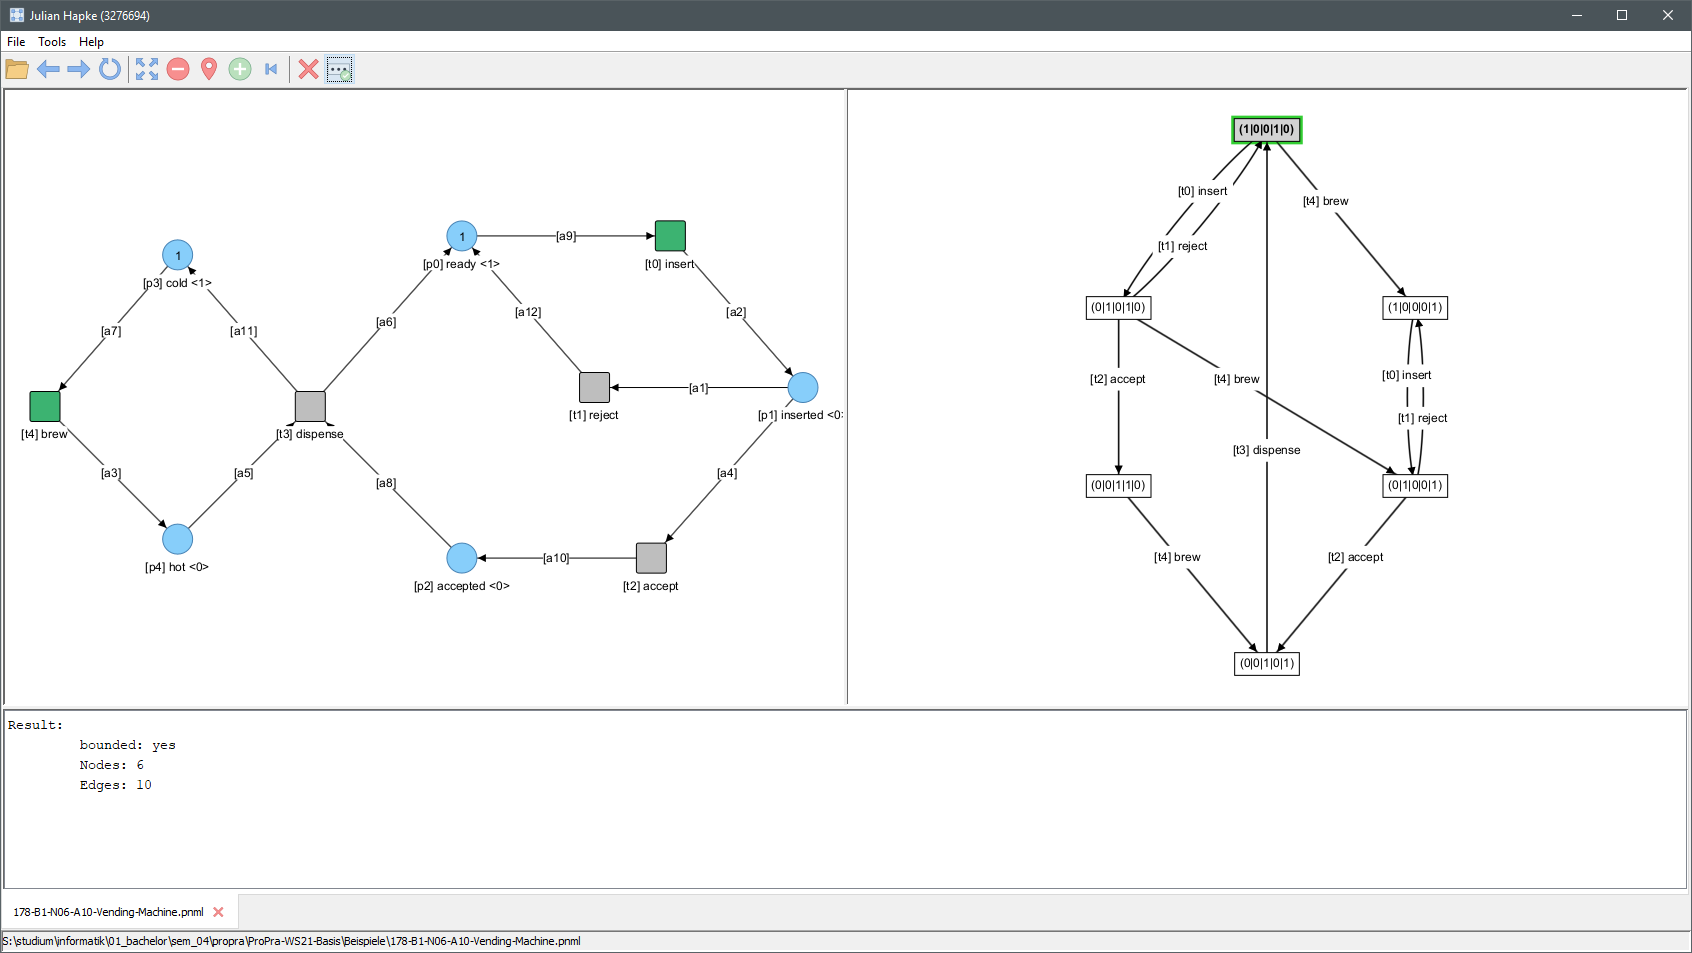
\includegraphics[width=\textwidth]{../img/Screenshot_178_hierarchy_layout.png}
  \caption{Beispieldatei 178 nach Beschränktheitsanalyse mit hierarchischem Layout}
  \label{img:ex178_hierarchy}
\end{figure}

\subsection{Einstellungen}
\label{sec:settings}
Nach dem Aufruf des Menüpunkt \emph{Extras $\rightarrow$ Einstellungen\ldots}
wird der in \cref{img:settings} dargestellt Dialog gezeigt.

\begin{figure}[ht]
  \centering
  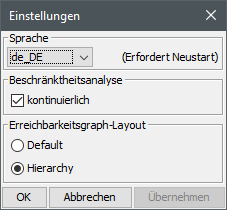
\includegraphics[width=0.3\textwidth]{../img/settings.png}
  \caption{Programmfenster nach dem Start}
  \label{img:settings}
\end{figure}

In diesem Dialog kann die Sprache der Oberfläche, die Warnung vor
Unbeschränktheit bei interaktivem Aufbau des Erreichbarkeitsgraphen und das
Layout der Darstellung des Erreichbarkeitsgraphen eingestellt werden. Die
Änderung der Sprache der Oberfläche bedarf eines Neustarts der Anwendung. Die
Änderung des Layouts des Erreichbarkeitsgraphen bedarf einer Neuerstellung des
Graphen, entweder durch Ausführen der Beschränktheitsanalyse oder Löschen des
aktuellen partiellen Erreichbarkeitsgraphen.
